\chapter{System Architecture}
\label{chap:architecture}

This chapter goes through the architecture of the closed-loop payment system. We start with the big picture, explain why we chose this approach over the alternatives, and then go into each component one by one. The whole idea behind the design is to keep things simple: one server, one app that works for everyone, and strive to have always network support. If network however will go down the balance will be always cached on the bracelet and used as a deciding factor if the payment will be approved or not. The system should be easy to deploy, easy to understand, and tough enough to handle what actually happens at a festival.

\section{High-level overview}
\label{sec:high-level-overview}

Most existing festival payment systems need a technical team to physically go to the venue, set up local servers, deploy a private network, and babysit the infrastructure for the entire duration of the event. As we discussed in Section~\ref{subsec:campus-cards}, the standard approach at festivals like Untold involves bringing dedicated servers on-site so that the payment logic runs locally. This makes sense when the balance lives on a remote server and every transaction needs a network round-trip to authorize. In that model, if the connection between the venue and the cloud drops, nobody can pay for anything, so you bring the server to the venue to avoid that dependency.

Our system takes a different path. As mentioned, we strive to always have reliable internet access using Starlink as the primary uplink, paired with a redundant network topology that keeps terminals talking to the server even when individual links degrade. The bracelet-as-cache fallback exists for the residual edge cases, but the goal is to never need it.

This means there is no need to deploy anything at the festival venue. No local servers, no private network infrastructure, no IT team on-site. The organizer creates an event through the admin dashboard, configures the parameters, approves the vendors, and distributes the wristbands. The vendors download the app, get whitelisted, and they are ready to accept payments. The server runs in the cloud, the same way it runs for every other festival on the platform. Nothing changes in the deployment.

The system has four main components: a backend server, a mobile application for attendees and vendors, a web-based admin dashboard, and NFC wristbands that carry the actual token balance for each attendee. The server is a single, multi-tenant service that manages all festivals from one deployment. There is no need to spin up a separate server or database for each event. An admin creates an event, configures it, and the system handles the rest. The mobile app is what attendees and vendors interact with: attendees see their balance and history, and vendors use it as a soft point-of-sale terminal. Admins manage the event through a separate web dashboard that works in any browser. The wristband is where the balance actually lives during the event.

Figure~\ref{fig:system-architecture} shows the high-level architecture of the system. The thing to notice is the NFC connection between the Vendor POS and the wristband at the bottom: that is the actual payment path, and it does not go through the server. Everything above that (the load balancer, the server instances, the database) is for management, reporting, and synchronization, not for processing individual payments.

\begin{figure}[ht]
	\centering
	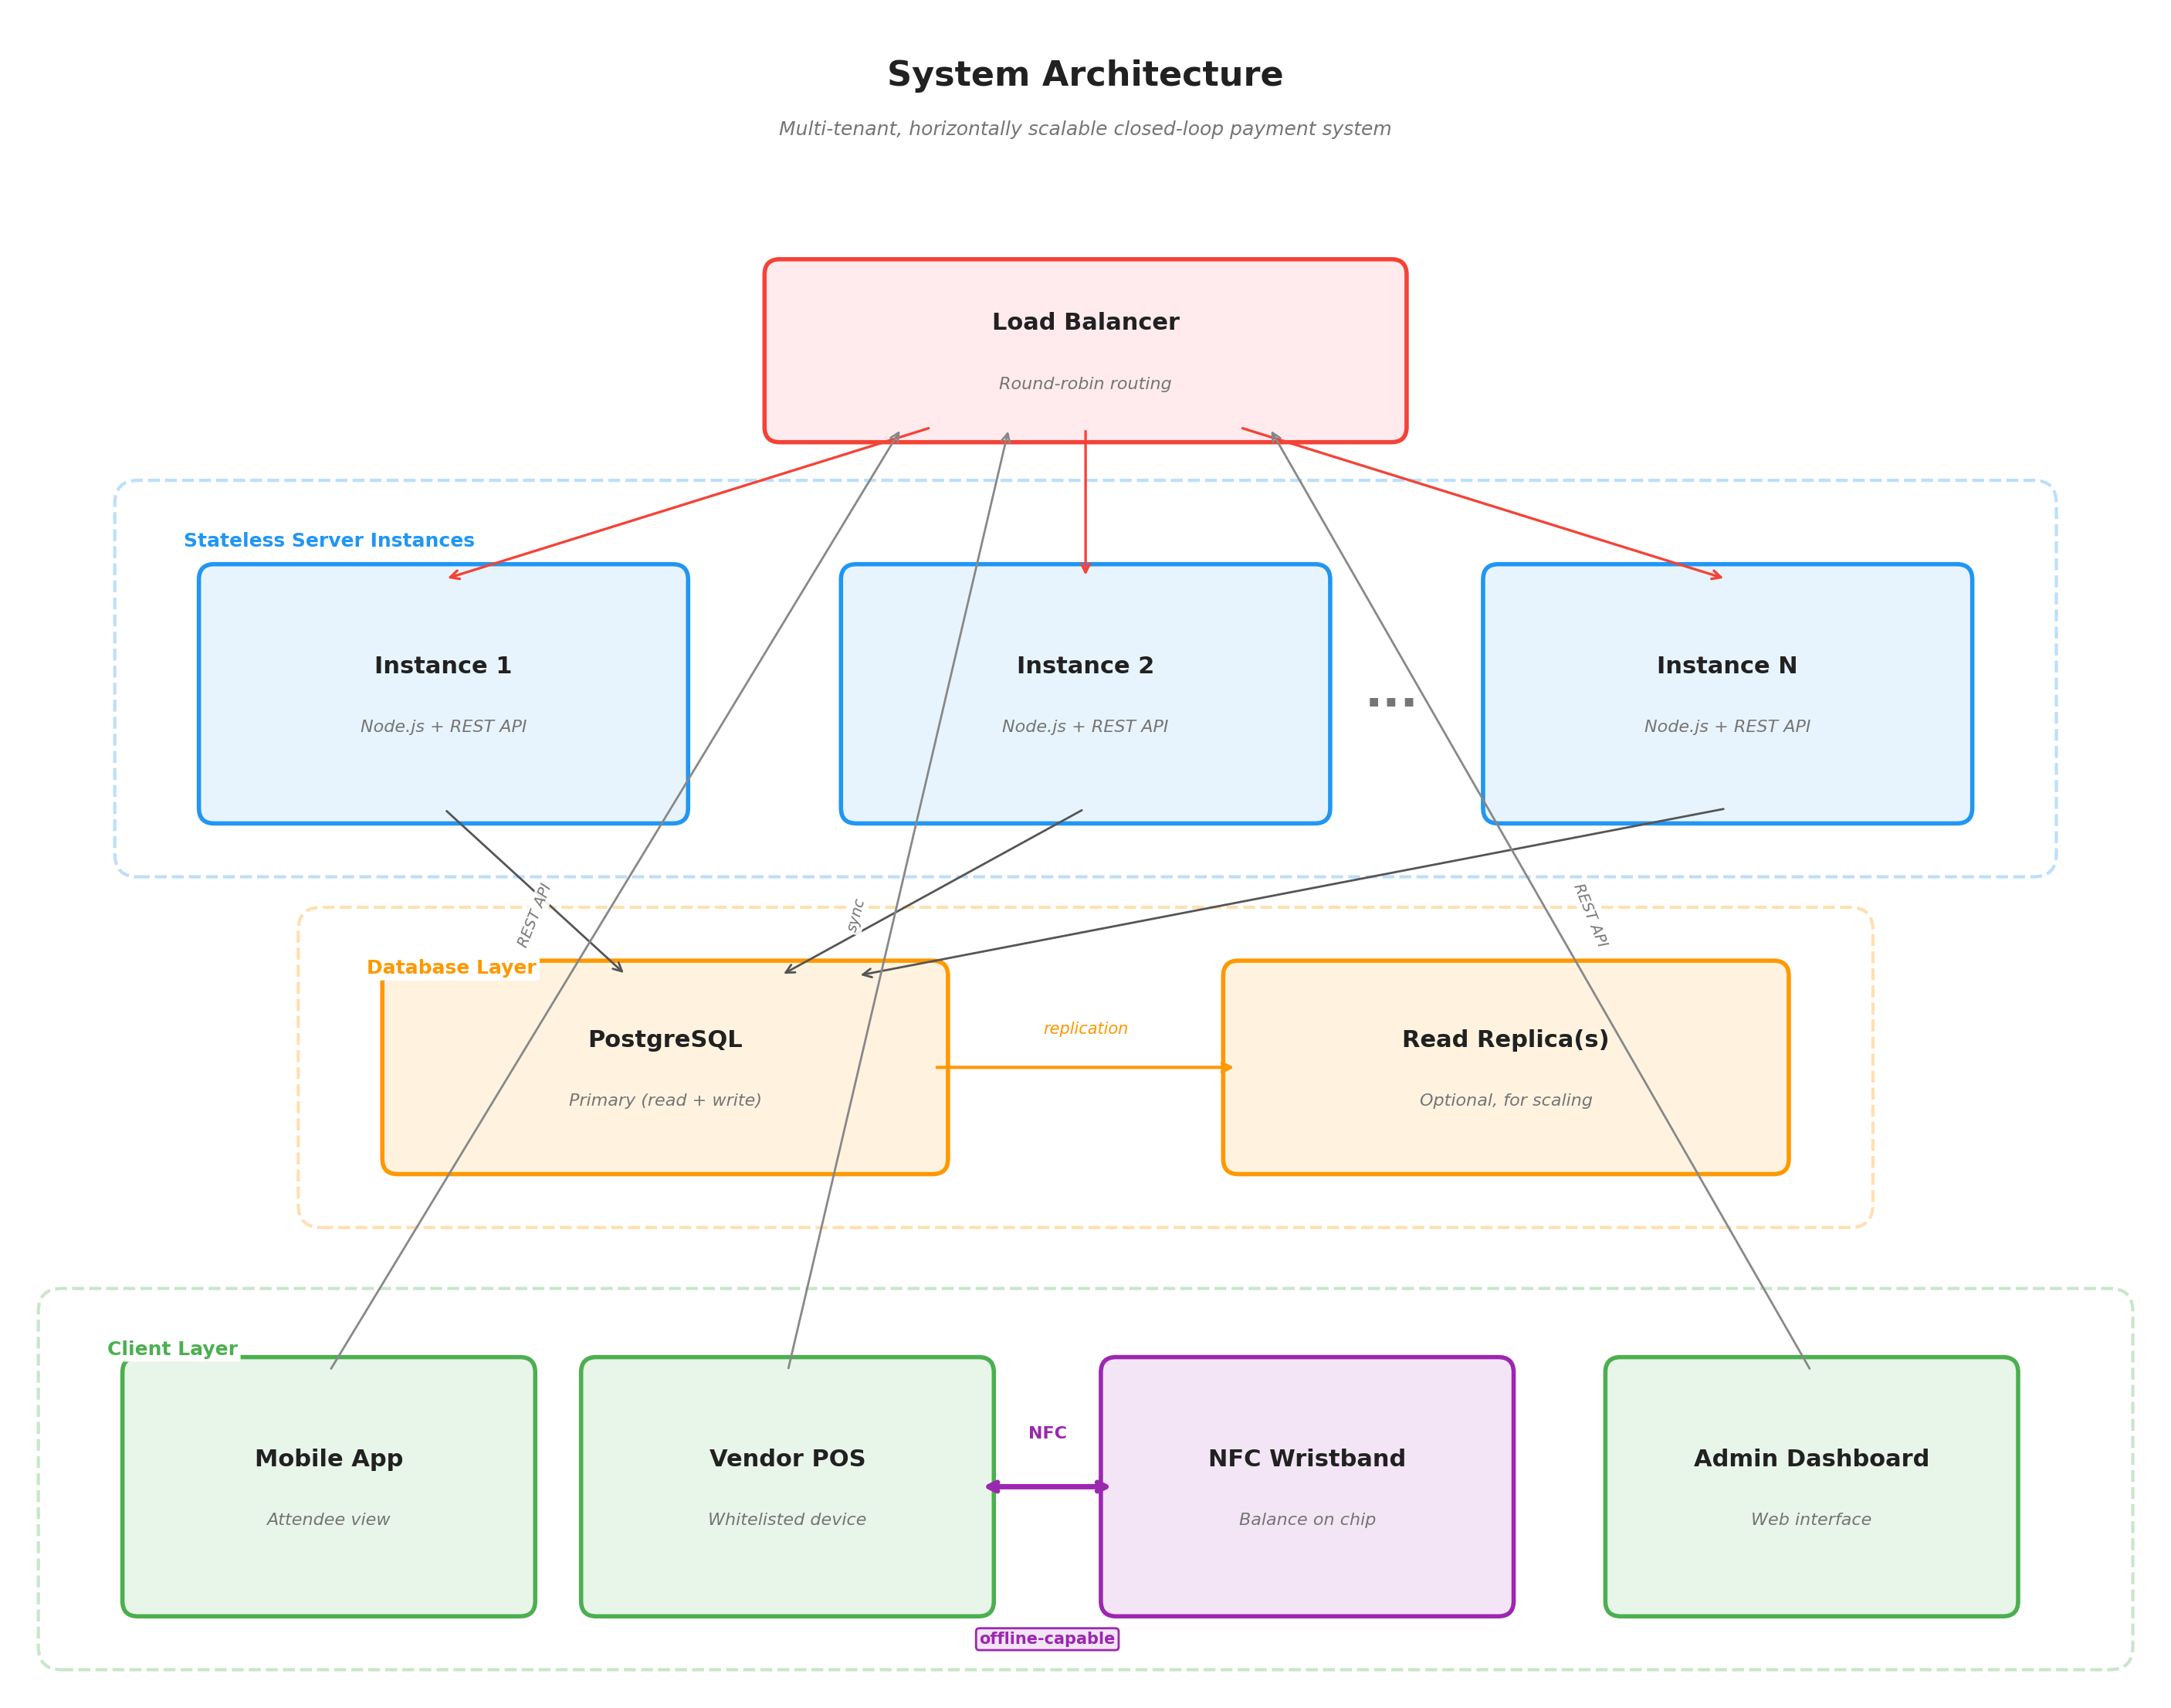
\includegraphics[width=0.95\textwidth]{images/system-architecture.png}
	\caption{High-level system architecture. Payments happen directly between the vendor device and the NFC wristband without server involvement. The backend handles event management, top-ups, and transaction log synchronization. Server instances are stateless and horizontally scalable behind a load balancer.}
	\label{fig:system-architecture}
\end{figure}

\section{Why this architecture}
\label{sec:why-architecture}

Before settling on this design, we considered a few different approaches and went through the techniques and patterns discussed in Chapter~\ref{chap:background} to figure out which ones are actually useful in our context and which ones would just add complexity for no real benefit. The choice of where the balance lives is really the decision that shapes everything else, so it is worth comparing the options side by side and explaining what we took from the literature and what we left behind.

\subsection{Architecture comparison}
\label{subsec:architecture-comparison}

\textbf{Option A: Server-side balance, online-only.} The wristband (or QR code, or whatever the attendee carries) is just an identifier. Every time a vendor scans it, the terminal sends a request to the server, which checks the balance, deducts the amount, and sends back a confirmation. This is the simplest model to reason about because the server is always the single source of truth. The problem is obvious: if the network goes down, payments stop completely. For a regular retail store this is fine because they have stable internet. For a festival with 50,000 people in a field, it is not.

\textbf{Option B: Server-side balance with local cache.} Same as Option A, but vendor terminals keep a cached copy of recent balances. When the network drops, they fall back to the cache. This sounds reasonable until you think about what happens when two vendors both have a cached balance of 50 tokens for the same user. Vendor A deducts 40, Vendor B deducts 40, and now the user has spent 80 tokens out of 50, caching the balance on the vendors devices still does not achieve anything if the cache is not shared between them.

\textbf{Option C: Balance cached on the wristband, server as source of truth.} The NFC chip on the wristband caches the user's balance, but the server remains the canonical record. In normal operation, vendors authorize against the server, which debits the balance and writes the updated value back to the chip. If connectivity drops, terminals fall back to the cached balance on the chip: they read it, verify funds, debit the chip, and queue the transaction locally for replay once the network returns. The user can only be in one place at a time, so the wristband naturally serializes transactions during offline periods, and a monotonic counter on the chip lets the server detect and apply queued debits in order without double-counting. This is the same principle that makes transit card systems like Suica and Octopus work: the card is fast and offline-capable, but the back office is always the authoritative ledger.

Table~\ref{tab:architecture-comparison} summarizes the comparison.

\begin{table}[ht]
	\centering
	\begin{tabular}{|l|c|c|c|}
		\hline
		\textbf{Criteria} & \textbf{A: Online-only} & \textbf{B: Cached} & \textbf{C: On wristband} \\
		\hline
		Works offline & No & Partially & Yes \\
		\hline
		Double-spend risk & None & High offline & None \\
		\hline
		Server dependency & Every tx & Every tx + cache & Sync only \\
		\hline
		On-site infrastructure & Required & Required & Not needed \\
		\hline
		Physical tamper risk & None & None & Needs secure chip \\
		\hline
		Complexity & Low & High & Medium \\
		\hline
	\end{tabular}
	\caption{Comparison of the three architectural approaches for storing the user balance.}
	\label{tab:architecture-comparison}
\end{table}

\subsection{What we learned from existing systems}
\label{subsec:lessons-existing}

In Chapter~\ref{chap:background} we looked at transit cards, commercial festival payment systems, and the EMV offline authorization model. Each one influenced our design in different ways.

Transit card systems like Suica and Octopus (Section~\ref{subsec:transit-cards}) are basically the proof that Option C works at scale. Suica processes millions of transactions per day with sub-second speed, all because the balance lives on the FeliCa chip and the gate does not need to call any server. Our wristband model takes the same core idea: the balance is on the chip, the terminal reads it, deducts, and writes back. The difference is that Suica runs on fixed gates maintained by professionals in train stations with dedicated private networks, while we run on random phones carried by festival vendors in a field. So the principle transfers, but the implementation details are quite different. We also borrowed the security model from FeliCa, specifically the mutual authentication between the chip and the reader, which we implement using MIFARE DESFire's AES-128 protocol instead of FeliCa's proprietary encryption. The idea is the same: both sides prove to each other that they are legitimate before any data gets exchanged.

From the commercial festival systems like Tappit and Intellitix (Section~\ref{subsec:campus-cards}), we mainly learned what we do not want to do. These systems require an IT team to go to the venue, set up local servers, deploy a private network, and manage the whole thing for the duration of the event. That works for a company with dedicated operations staff, but it does not work if the goal is a system that a small organizer can deploy by themselves. The conversations we had with people who worked on the Untold deployment confirmed this: even with dedicated on-site infrastructure, top-up synchronization delays of two to four hours were common when the Wi-Fi got bad. Our architecture avoids this entirely because there are no on-site servers to maintain. The wristband handles payments locally, and the cloud server only needs to be reachable for top-ups and sync, which can tolerate delays without blocking the actual payment flow.

The EMV offline authorization model (Section~\ref{subsec:emv}) gave us the idea of using spending limits as a risk control mechanism. EMV cards carry parameters that define how much they can spend offline before they have to go online for authorization. We use a similar concept: the event admin can configure maximum transaction amounts and maximum total offline spend per wristband. This is mostly relevant as a safety net for the edge case where someone does manage to tamper with a wristband, it limits the potential damage. But unlike EMV, where the card self-reports its own state and the terminal has to trust it (which, as Murdoch et al.~\cite{Murdoch2010} showed, is exploitable), our DESFire wristbands authenticate cryptographically before every read and write. The terminal does not take the wristband's word for it, it verifies through the shared AES key.

\subsection{What we took from the architectural patterns}
\label{subsec:lessons-patterns}

In Section~\ref{sec:offline-first} we covered several architectural patterns for offline operation: local-first software, CRDTs, event sourcing with CQRS, and edge computing. Not all of them ended up being useful for our case.

\textbf{Local-first software} (Section~\ref{subsec:local-first}) is a nice philosophy, but as we discussed in Chapter~\ref{chap:background}, it does not fit payment systems well. Kleppmann et al.~\cite{Kleppmann2019} designed it for collaborative applications where merging conflicting edits is annoying but acceptable. With money, you cannot just merge two conflicting balance updates and hope for the best. Our system borrows the basic idea of keeping a local copy of data so the app works without the network, but the server remains the source of truth and offline transactions are treated as provisional. It is a weaker version of local-first, and that is the right call for a system where financial correctness actually matters.

\textbf{CRDTs} (Section~\ref{subsec:crdts}) are an interesting solution for data convergence in distributed systems, but they turned out to be overkill for what we need. CRDTs guarantee that all replicas converge to the same value regardless of the order updates arrive, which sounds great until you realize they cannot enforce constraints like ``the balance must not go below zero.'' In our case, since the balance lives on the wristband, we do not really have a distributed data convergence problem in the first place. The wristband is the single copy of the balance during the event. There is nothing to converge. The server's copy is just a log of what happened, reconstructed from the transaction events that vendor devices upload. So CRDTs would add complexity to solve a problem that our architecture does not have.

\textbf{Event sourcing} (Section~\ref{subsec:event-sourcing}) is the one pattern we actually use directly. Every transaction that happens on a vendor device is recorded as an immutable event with a timestamp, a device ID, a wristband ID, and the amount. When the device is online, these events are sent to the server immediately. When it is offline, they queue up locally and get pushed as a batch when connectivity returns. The server reconstructs the state of each wallet by replaying these events. This gives us a full audit trail of everything that happened, which is important for settlement and for the event organizer to see where the money went. We do not use CQRS in the formal sense (separate read and write models), but in practice the vendor app does maintain a local read cache of recent transactions that is separate from the write queue, which is a similar idea.

\textbf{Edge computing} (Section~\ref{subsec:edge-computing}) shows up in our architecture at two levels. The first and more obvious one is the vendor phones themselves. Each phone runs the payment logic locally: read the wristband, validate the balance, deduct, write back. The cloud server coordinates and collects data, but it is not in the critical path of a payment. We also pushed the state further out than a typical edge setup, all the way to the wristband itself, so the edge node (the phone) does not even need to maintain a local copy of the balance. It reads the authoritative state directly from the chip every time. The second level is the server deployment itself. We deploy on Railway, which lets us pick the region where the container and the database run. So for festivals in Romania or elsewhere in Europe, the backend sits in a European data center with low latency to the vendor devices, instead of routing everything through some server in the US. For the operations that do need the server (top-ups, sync, admin dashboard), this makes a noticeable difference in responsiveness. And if the platform ever expands to other continents, spinning up another region on Railway is just a configuration change, no need to touch the application code.

\textbf{The CAP theorem} (Section~\ref{subsec:cap-theorem}) told us what we already knew intuitively: during a network partition at a festival, we have to choose between consistency and availability, and refusing transactions because the Wi-Fi dropped is not acceptable. Our architecture sidesteps the hardest part of this tradeoff by putting the balance on the wristband. With Option B (server-side balance with cache), you are fully in CAP territory because the cached balances on different terminals can diverge and you get double-spend. With Option C (balance on wristband), the wristband itself acts as a single, physically consistent copy that moves with the user. There is no partition between the balance and the terminal that is reading it, because they are in direct NFC contact. The CAP tradeoff still applies to the synchronization of transaction logs with the server, but there the worst case is delayed reporting, not double-spending, which is a much smaller problem.

So to sum it up: from the existing systems we took the on-chip balance model (transit cards), spending limits as a safety net (EMV), and the lesson that on-site infrastructure should be avoided (festival systems). From the architectural patterns, we took event sourcing for the transaction log and edge computing as the general execution model, but we left behind local-first's strong local ownership model and CRDTs because the wristband balance model makes them unnecessary.

\section{NFC wristbands and offline support}
\label{sec:wristband-offline}

Since the balance lives on the wristband, the offline story becomes much simpler than it would be with a server-side model. This section explains how the wristband interaction works, what happens during offline periods, and how the system reconciles everything once connectivity comes back. We also touch on the security considerations here, because with the balance stored physically on the chip, security is part of the architecture, not something you bolt on afterwards.

\subsection{How a payment works}
\label{subsec:how-payment-works}

The transaction flow between the vendor device and the wristband goes like this:

\begin{enumerate}
	\item The vendor enters the amount (or selects items from a product catalog) on their phone.
	\item The customer taps their wristband against the phone's NFC reader.
	\item The app reads the current balance and transaction counter from the wristband.
	\item The app checks that the balance is sufficient.
	\item The app writes the new (lower) balance and an incremented counter back to the wristband.
	\item Only after a successful write confirmation, the transaction is recorded as completed in the local log.
	\item If the write fails (customer pulled their wrist away too quickly, interference, etc.), the transaction is marked as failed and the vendor is prompted to retry.
\end{enumerate}

This ordering is important. The vendor device never records a successful payment unless the wristband was actually updated. The worst case scenario is that the vendor has to ask the customer to tap again, which is a small inconvenience but not a financial problem.

\subsection{Offline operation}
\label{subsec:offline-operation}

During normal online operation, vendor terminals send each transaction to the server right after it is recorded locally. The server updates its own ledger, which is the authoritative record for reporting, settlement, and auditing.

When the network goes down, vendor terminals keep processing payments exactly as before. The wristband interaction does not change at all. The only difference is that transactions accumulate in the local queue on the vendor device instead of being sent to the server. Once connectivity returns, the device pushes its queued transactions to the server in a batch.

\subsection{Balance reconciliation model}
\label{subsec:balance-reconciliation}

A closed-loop payment system with offline-capable terminals has two writers that can mutate balance state: the server (when users top up) and the chip (when users pay vendors). During a network partition, both can act independently, and the system has to converge on a correct final state once connectivity is restored. This is a well-studied problem in distributed systems, and naive solutions tend to either double-spend, double-credit, or lose money in subtle ways.

Our model relies on a strict separation of concerns between the two writers. The server is the only writer for credits (top-ups, refunds, adjustments). The chip is the only writer for debits (vendor payments). Because the two operation types live in disjoint lanes, no merge conflict is possible: addition and subtraction commute, and each lane has exactly one authoritative source. We require top-ups to be online-only, which keeps the credit lane fully under server control and avoids the entire class of problems that arise when both sides can issue credits independently.

\subsubsection{State and counters}

Each wristband stores four fields: \texttt{balance} (the cached balance in minor units), \texttt{debit\_counter} (a monotonic counter incremented on every chip-side debit), \texttt{credit\_counter\_seen} (the highest server-side credit sequence the chip has acknowledged), and identity fields (\texttt{bracelet\_uid}, \texttt{event\_id}) written at provisioning.

The server maintains per-wallet: \texttt{balance} (the canonical balance), \texttt{credit\_counter} (incremented on every server-side credit), and \texttt{debit\_counter\_seen} (the highest debit counter value the server has reconciled from any terminal).

The two counters are independent monotonic sequences, each with a single writer. The chip owns \texttt{debit\_counter}; the server is a read-only mirror via \texttt{debit\_counter\_seen}. The server owns \texttt{credit\_counter}; the chip is a read-only mirror via \texttt{credit\_counter\_seen}. Because each lane has exactly one writer, there is never a merge conflict within a lane.

\subsubsection{Invariants}

The correctness of the model rests on two invariants that must hold at all times:

\begin{enumerate}
	\item \textbf{The chip never increases its own balance.} Every chip-side mutation is a debit: \texttt{balance -= amount} and \texttt{debit\_counter += 1}, performed atomically by the secure element.
	\item \textbf{The server is the only source of credits.} Top-ups, refunds, and adjustments mutate \texttt{server.balance} and increment \texttt{credit\_counter}. The chip picks up these credits passively on the next tap.
\end{enumerate}

As long as these two invariants hold, the chip and server cannot disagree about who added money or who spent it. Reconciliation reduces to a union of two non-conflicting streams.

\subsubsection{Operations}

\textbf{Top-up (always online).} The server increments \texttt{balance} and \texttt{credit\_counter}, writes a transaction row, and acknowledges. The chip is not touched. The user's chip is now stale relative to the server, but this is harmless: the next tap will reconcile.

\textbf{Online debit.} The terminal reads the chip and forwards the request to the server with the chip's current \texttt{debit\_counter} and \texttt{credit\_counter\_seen}. The server checks for pending credits (any with sequence number greater than \texttt{credit\_counter\_seen}) and applies them as part of the same response. It then validates the debit, updates its own ledger, and returns the new triple \texttt{(balance, debit\_counter, credit\_counter\_seen)} to the terminal, which writes it atomically to the chip. Pending credits and the new debit are picked up by the chip in a single round trip.

\textbf{Offline debit.} The terminal reads the chip, verifies sufficient balance, and performs an atomic decrement on the chip's value file. It generates an idempotency key before any network attempt, queues the transaction locally with the resulting \texttt{debit\_counter} value, and serves the customer. The terminal continues to drain its queue in the background as connectivity allows.

\textbf{Sync.} When a terminal regains connectivity, it pushes queued transactions to the server in batches. The server applies them idempotently using the per-transaction key, updates \texttt{wallet.balance}, and advances \texttt{debit\_counter\_seen} to the highest counter value observed. Because debits are subtraction and the chip already enforced no-overdraft at the moment of each debit, the server can apply queued transactions in arrival order without strict sequencing.

\subsubsection{Concurrent top-up and offline debit}

Consider the canonical hard case. A user starts with chip \texttt{(50, debit=6, credit\_seen=0)} and server \texttt{(50, credit=0, debit\_seen=6)}. The user pays 10 tokens at an offline terminal, taking the chip to \texttt{(40, debit=7, credit\_seen=0)}. Concurrently, a 20-token top-up lands on the server, taking it to \texttt{(70, credit=1, debit\_seen=6)}. Both sides have advanced in their own lane. Both are correct.

When the user taps an online terminal, the terminal reads \texttt{(40, 7, 0)} from the chip and forwards it to the server. The server observes that \texttt{credit\_counter=1} is greater than \texttt{credit\_counter\_seen=0}, meaning there is one pending credit of 20 tokens to apply. It also observes that \texttt{debit\_counter=7} is greater than \texttt{debit\_counter\_seen=6}, meaning there is one chip-side debit it has not yet seen, but it does not need to know the amount to safely apply the credit. The server writes \texttt{(60, 7, 1)} to the chip. When the offline terminal eventually syncs the queued -10 debit, the server applies it: \texttt{balance: 70 - 10 = 60, debit\_counter\_seen=7}. Both sides converge to 60 tokens. No conflict resolution was needed because the two streams never collided.

\subsubsection{Lost transactions}

The model does not magically prevent loss. If a terminal dies before draining its queue, the vendor has served the customer and the chip has correctly subtracted the amount, but the server has no record of the transaction. The detection mechanism is automatic: when the server observes that \texttt{chip.debit\_counter} exceeds \texttt{debit\_counter\_seen} plus the count of pending queued transactions tracked server-side, the gap represents lost transactions.

The resolution policy is to trust the chip's balance immediately (the chip's atomic decrement is authoritative), wait a configurable grace period for late syncs, and after expiry reconcile by writing the chip's balance to the server and logging the discrepancy for ops review. The festival absorbs the loss for those specific transactions; vendors with local receipts can claim manually if the amount is worth chasing.

The exposure is bounded by the sync interval. With terminals syncing every 30 seconds, the worst-case loss per dead terminal is roughly \texttt{sync\_interval} times \texttt{peak\_tps} times \texttt{avg\_tx\_value}, on the order of low hundreds of euros per terminal failure. This is a tractable operational risk rather than a correctness problem.

\subsubsection{Why this model}

The design borrows from established patterns in closed-loop transit systems (Suica, Octopus, Oyster) and EMV offline authorization, where the card is authoritative for offline operations and the back office reconciles with bounded operator-absorbed risk. Compared to a single-counter approach, the two-counter scheme avoids a known correctness bug where chip and server can have equal counters but divergent state due to concurrent operations in different lanes. Compared to a full vector clock or CRDT, it is dramatically simpler because the strict lane separation makes a 2-dimensional clock degenerate into two independent scalars. The result is a model that is correct under all realistic failure modes, requires no exotic distributed systems primitives, and maps cleanly to the chip's hardware capabilities.

\subsection{Top-ups: the one thing that needs the network}
\label{subsec:topups}

Topping up is the one operation that cannot happen offline. When an attendee loads tokens onto their wristband, real money needs to move from their bank account through Stripe and into the event operator's account. This requires an internet connection. Restricting top-ups to online-only is also what keeps the credit lane fully under server control, which is the foundation of the reconciliation model described above.

Top-ups can happen in two ways. First, attendees can top up through the app before or during the event, using Stripe. Once the payment clears, the server records the new balance and increments \texttt{credit\_counter}. The attendee does not need to do anything special: the next time their wristband is read by any vendor terminal (online), the pending credit is picked up automatically and written to the chip as part of that interaction. Second, dedicated cash top-up stations at the event take cash and submit the credit through the server, which then writes the new balance to the wristband on the spot. In both cases, the server is the only writer of credits, and the chip only ever receives credits via an authenticated server response.

\subsection{Security of the wristband balance}
\label{subsec:wristband-security-intro}

Storing the balance on the wristband opens up questions that you do not have with a server-side model. If the balance is just a number written to an NFC chip, what stops someone from using their phone to give themselves more tokens?

The answer depends on the chip. Cheap MIFARE Classic chips, as Garcia et al.~\cite{Garcia2008} demonstrated, have broken encryption and can be cloned or modified without too much effort. This is why we use MIFARE DESFire EV2 or EV3 chips, which support AES-128 encryption and mutual authentication between the chip and the reader. With these chips, writing to the balance requires a secret key that is stored securely on both the chip and the vendor terminal. Without the key, you cannot modify the balance.

There are three main threats we need to address:

\textbf{Balance tampering.} Someone tries to modify the balance on their wristband to give themselves more tokens. With DESFire EV3, all read and write operations on the relevant data files require authentication with the AES key. The chip itself enforces this at the hardware level, so even if someone has physical access to the wristband and a phone with an NFC reader, they cannot change the balance without knowing the key.

\textbf{Cloning.} Someone tries to copy their wristband onto another chip so they can use the same balance twice. DESFire chips have a unique, factory-programmed identifier (UID) that cannot be changed or duplicated. The system can bind the balance data to this UID, so even if someone managed to copy the data files (which they cannot without the key), the clone would have a different UID and would be rejected by the vendor terminal.

\textbf{Secure communication with the soft POS.} The vendor's phone acts as the POS terminal, and the communication between the app and the NFC chip needs to be protected. DESFire EV3 supports secure messaging, which means the data exchanged between the chip and the reader is encrypted and authenticated in both directions. An attacker cannot eavesdrop on the NFC communication to extract the key, and cannot inject fake commands to the chip.

Each transaction also includes a rolling counter (the \texttt{debit\_counter} described in Section~\ref{subsec:balance-reconciliation}) that chains transactions together. If someone did manage to tamper with the balance somehow, the chain would break, and the system would detect it the next time the wristband is scanned by a legitimate terminal.

We discuss these security considerations in much more detail in Chapter~\ref{chap:security}, including the threat model, the key management strategy, and what happens when the system detects a compromised wristband.

\section{The mobile application}
\label{sec:mobile-app}

There is one mobile app, built in React Native, that attendees and vendors both download. What the user sees depends on their role: attendees see their balance, and vendors get a POS terminal. The reason we went with React Native is that the same codebase needs to run on both regular phones (for attendees checking their balance) and on the devices that vendors use as POS terminals. We did not want to maintain two separate apps, and React Native gives us one codebase that compiles to both iOS and Android. Since the vendor POS is just a phone with NFC capabilities, the same app handles both use cases. The admin dashboard is a separate React web application, which we cover in Section~\ref{sec:admin-dashboard}.

\subsection{Attendee view}
\label{subsec:attendee-view}

Attendees see a simple screen showing their current token balance, a transaction history list, and a way to top up their wallet online using Stripe. The balance displayed in the app is synced from the server and shows the last known state. However, the real balance during the event lives on the wristband, not in the app. The app is mostly informational for attendees: it is nice to check your balance and see what you spent, but the actual payment happens by tapping the wristband at a vendor terminal.

\subsection{Vendor POS mode}
\label{subsec:vendor-pos}

When an admin has whitelisted a device from the admin dashboard, the app switches to POS mode on that device. The vendor sees a payment screen where they enter the amount (or select items from a product catalog), and then the customer taps their wristband against the phone's NFC reader. The app reads the balance, checks that there are enough tokens, deducts the amount, writes the new balance back, and logs the transaction locally. If the device is online, the transaction is also sent to the server immediately. If not, it goes into the local queue and gets synced later.

To become a vendor, the business needs to provide basic information: business name, a contact person, and the type of products they sell. The admin reviews this and can approve or reject the application. Once approved, the admin whitelists specific devices (identified by their device ID) as POS terminals for that vendor. This whitelisting step matters because it means not just any phone can start accepting payments. Only devices that the admin has explicitly authorized will have the POS functionality enabled.

\subsection{Device security checks}
\label{subsec:device-security}

Since the vendor's phone is effectively a payment terminal, the app needs to check some basic security measures before allowing POS mode. A rooted or jailbroken phone is a risk because someone could modify the app to skip the balance check or tamper with the transaction logs. The app checks for root/jailbreak status at startup and refuses to enter POS mode on compromised devices.

Beyond root detection, the app also verifies that it is running the official, unmodified version (not a repackaged APK), that the device has a screen lock enabled, and that the OS version is not critically outdated. These are not bulletproof checks (determined attackers can bypass root detection), but they raise the bar enough to prevent casual tampering and give the system a way to flag suspicious devices to the admin.

\section{Admin dashboard}
\label{sec:admin-dashboard}

The admin dashboard is a separate web application built in React, not part of the mobile app. We made it a website so that any event organizer can access it from any device with a browser, without needing to download anything. This also means it works on laptops, tablets, or phones, whatever the admin has on hand. The dashboard covers four main areas:

\textbf{Event setup.} The admin creates the event, sets the token-to-currency exchange rate, defines spending limits, configures the commission rates for vendors, and sets the event dates. The event goes through a lifecycle (setup, active, settlement, closed) and the dashboard controls the transitions between phases.

\textbf{Vendor and device management.} The admin reviews vendor applications, approves or rejects them, and whitelists specific devices as POS terminals. Each vendor can have multiple devices, and the admin can see which devices are currently active, when they last synced, and how many transactions they have processed.

\textbf{Monitoring and statistics.} During the event, the dashboard shows real-time transaction volume (when devices are online), total tokens in circulation, revenue by vendor, and a timeline of sync events. This gives the organizer visibility into how the event economy is performing.

\textbf{Security monitoring.} The dashboard flags suspicious activity: devices that have not synced in a long time, wristbands with transaction chain breaks (potential tampering), devices that failed root detection checks, and any balance discrepancies flagged during reconciliation. The admin can block a device or wristband directly from the dashboard if something looks wrong.

\section{Backend server}
\label{sec:backend-server}

The backend is built with NestJS, a Node.js framework that gives us a structured way to organize the codebase into modules. We chose NestJS because it enforces a clean separation between controllers (handling HTTP requests), services (business logic), and repositories (database access), which keeps the code organized as the project grows. It also has built-in support for things like guards (for authentication), interceptors (for logging and error handling), and dependency injection, which would otherwise require setting up manually with a bare Express or Fastify server.

The server is deployed as a Docker container on Railway, which gives us a managed PostgreSQL database in the same region as the container. We deploy to a European region so that the latency between the vendor devices and the server stays low for festivals in Romania and the rest of Europe.

The server exposes a REST API that covers four main areas: authentication and accounts (registration, login, token refresh, role-based access control), event management (creating and configuring events, managing the event lifecycle), vendor management (approving vendors, whitelisting devices, setting commissions), and sync/reconciliation (endpoints for vendor devices to push their offline transaction logs and pull updated state).

\subsection{Why a single service, not microservices}
\label{subsec:why-monolith}

It would be tempting to split the backend into separate services for payments, event management, and synchronization. But for our use case, splitting introduces problems without solving any real ones.

If the payment service needs to check whether a vendor is authorized for an event before processing a sync, and that information lives in a different service, we now have distributed transactions or eventual consistency between our own services. That is exactly the kind of complexity we are trying to avoid. With a single service, a database transaction can atomically check the vendor status and record the payment in one go.

The practical argument is also about operations. Nobody wants to manage five services, five deployment pipelines, and five sets of logs for what is fundamentally one product. With a single service, the entire platform runs as one container image plus a PostgreSQL database. Deploying a new version means rolling out one image. Debugging a production issue means looking at one set of logs. This simplicity is not just convenient, it is what makes it realistic for a small team (or one person, in the case of this thesis) to actually run the thing.

This does not mean the code is a mess internally. NestJS modules give us the same logical separation that microservices would, just without the network boundary between them. The payment module, the event module, and the sync module each have their own services, controllers, and DTOs. If someday the platform grows to the point where splitting makes sense, the module boundaries are already there.

\subsection{Multi-tenancy}
\label{subsec:multi-tenancy}

The server handles all festivals from a single deployment. Every table in the database is scoped by an \texttt{event\_id} column, which acts as the tenant boundary. When a vendor device makes an API call, the request includes the event context (through a path parameter or a token claim), and all queries are filtered by that event. Data from Festival A is never visible to users of Festival B, even though it all lives in the same database.

This is simpler and cheaper than deploying a separate server and database for each festival. With per-festival deployments, the operator would need to provision infrastructure before each event, manage dozens of database instances, handle migrations across all of them, and tear everything down afterwards. With multi-tenancy, adding a new festival is just creating a row in the events table.

\subsection{Horizontal scalability}
\label{subsec:horizontal-scalability}

Keeping the server as a single service does not mean it is limited to a single instance. The server is designed to be stateless: it stores no session data or cached state in memory. Every request gets everything it needs from the database and from the JWT token in the request header. This means we can run as many instances of the server as we want behind a load balancer, and any instance can handle any request. There are no sticky sessions, no in-memory caches to synchronize, and no inter-instance communication.

For most festivals, a single instance will be more than enough. The majority of transactions during the event happen on the wristband itself without touching the server at all. The server mostly handles top-ups (which are less frequent), sync batches from vendor devices (which are periodic, not per-transaction), and admin dashboard queries. But if the platform grows to the point where dozens of festivals are running simultaneously and the sync traffic gets heavy, scaling horizontally is just a matter of increasing the replica count.

\section{Database: PostgreSQL}
\label{sec:database}

The database is PostgreSQL, and we are running a single instance of it (with the option to add read replicas later if needed). The schema is intentionally simple: users, events, wallets (one per user per event), transactions, and a sync log that tracks which device uploaded what and when.

\subsection{Why PostgreSQL}
\label{subsec:why-postgres}

PostgreSQL gives us ACID transactions for the financial data and is mature enough that we do not have to worry about edge cases in the transaction isolation. For a payment system, this matters. When the server processes a top-up, it needs to atomically check the Stripe payment status, create the transaction record, and update the wallet balance. If any step fails, everything rolls back. With PostgreSQL, this is just a regular database transaction.

\subsection{Why a single database is enough}
\label{subsec:single-database}

A common worry with using one database for everything is whether it can handle the load. But the reality is that PostgreSQL can handle a lot more than people give it credit for. The best example is probably OpenAI. In January 2026, they published a blog post~\cite{OpenAIPostgres2026} describing how they run ChatGPT, a product with over 800 million users, on PostgreSQL. Their setup is a single primary PostgreSQL instance on Azure that handles all writes, with around 50 read replicas spread across multiple regions for reads. The whole thing processes over a million queries per second while keeping p99 latency in the low double-digit milliseconds and maintaining five-nines availability. They did not shard the database or switch to some exotic distributed database. They scaled PostgreSQL with read replicas, connection pooling, query optimization, and by offloading write-heavy workloads to separate sharded systems when needed.

If that setup can serve 800 million ChatGPT users, a festival payment system with 50,000 attendees is not going to be the thing that breaks PostgreSQL. And in our case, the database load is even lighter than a typical web application. Most payment transactions happen entirely on the wristband and never touch the database in real time. The database mainly handles top-ups, periodic sync batches from vendor devices, and dashboard queries. Even during a large festival, the peak database load is modest because the actual payment processing is offloaded to the wristband.

If the platform does grow to the point where the database becomes the bottleneck, we can follow the same playbook that OpenAI used: add read replicas for distributing query load, use connection pooling (PgBouncer) to handle many concurrent connections efficiently, and partition tables to keep query performance stable as the data grows. These are all standard operational techniques that do not require changing the application code.

